\documentclass{book}
%%%%%%%%%%%%%%%%%%%%%%%%%%%%%%%%%%%%%%%%%%%%%%%%%%%%%%%%%%%%%%%%%%%%%%%%%%%%%%%%%%%%%%%%%%%%%%%%%%%%%%%%%%%%%%%%%%%%%%%%%%%%%%%%%%%%%%%%%%%%%%%%%%%%%%%%%%%%%%%%%%%%%%%%%%%%%%%%%%%%%%%%%%%%%%%%%%%%%%%%%%%%%%%%%%%%%%%%%%%%%%%%%%%%%%%%%%%%%%%%%%%%%%%%%%%%
\usepackage[cip,ChapterTOCs]{krantz_new}
\usepackage{times,mathptmx}
\usepackage{graphicx}
\usepackage{makeidx}
\usepackage{url}
\usepackage{amsmath}
\usepackage{amsfonts}
\usepackage{float}
\usepackage{paralist}
\usepackage{subfig}

\makeatletter
\renewcommand{\@cite}[1]{#1}
\def \@biblabel#1{\hspace*{-\labelsep}}
\makeatother
\setcounter{secnumdepth}{2}
\setlength{\parindent}{0in}
\parskip \medskipamount
\newcommand{\textcode}[1]{\textsf{\small #1}}   % always format something that could be written in matlab the same way

\begin{document}

% must set chapter counter to previous chapter
\setcounter{chapter}{8}

\chapter{Learning Algorithms}

\markboth{Information Complexity Toolbox for MATLAB}{Information
Complexity Toolbox for MATLAB}

In this chapter we present two classes of learning algorithms.
We begin with the genetic algorithm, which lends itself well to
many statistical modeling and optimization problems, such as
variable subsetting, mixture modeling, and maximum likelihood
estimation. After that we detail a function implementing
simulated annealing, though it does not seem as valuable a
statistical modeling tool as the genetic algorithm.

\section{Introduction}

The first part of this chapter is dedicated to the genetic algorithm; the
value of this optimization technique is demonstrated in two contexts -
variable subsetting and maximum likelihood estimation. The genetic algorithm
(GA) is a stochastic search procedure that borrows concepts from biological
evolution. Biological chromosomes, which determine so much about organisms,
are represented as binary words -- these determine the composition of
possible solutions to an optimization problem. As an example, consider a
subsetting problem such as would occur in multivariate regression: each
solution is a q-length vector such that each locus represents the presence
(1) or absence (0) of a specific predictor. An example may be $%
\begin{bmatrix}
1 & 0 & 0 & 1 & 1 & 0 & 0 & 1%
\end{bmatrix}%
$; in this case, predictors 1,4,5,8 will be used for OLS while 2,3,6,7 will
not. In the context of a numerical optimization problem, the chromosomes
represent a real value. Consider the problem of finding the MLE for some
single parameter distribution where we have reason to believe the maximum $%
\hat{\theta}$ lies in the interval $\left( \theta _{L},\theta
_{U}\right) $. We can use this information to encode real
values in this range as binary chromosomes. For example, say
our interval is $\left( -10,10\right) $, and
we want to use $B=8$ bits. The real value $x=3.6$ would be encoded as $%
\begin{bmatrix}
1 & 0 & 1 & 0 & 1 & 1 & 0 & 1%
\end{bmatrix}%
$.

Each iteration of the GA is called a \emph{generation}; maintaining the
biological analogy, each generation is composed of a \emph{population} of
solutions called \emph{individuals} - all represented by binary \emph{%
chromosomes}. Within a generation, individuals are allowed to perpetuate
their genes by mating; with whom they mate, and the frequency with which
they mate is determined by their \emph{fitness} as defined by some \emph{%
objective function}. Unlike the biological analogy, mating always produces
two offspring, so the population remains of a constant size (more this
paragraph). When two individuals mate, there is a certain probability that
their chromosomes will trade portions, through a \emph{crossover} operation;
this probability is usually set rather high ($0.75$ for example). When
members of the current generation procreate, there is a typically small
probability ($0.10$ for example) that some spots (\emph{loci}) on the
offspring's chromosomes will \emph{mutate}: $1\longrightarrow 0$ or $%
0\longrightarrow 1$. The benefit of the mutation operator should be clear,
without it, the GA would suffer from the main pitfall of most search
procedures: that of getting stuck in local optimum. Even if a next
generation ended up completely homogenous after crossover, mutation would
widen the search by allowing a jump to another area of the fitness
landscape. In real life, it can occasionally happen that an especially fit
individual will remain a desirable partner for more than one generation;
think Sean Connery, Harrison Ford, or Charlton Heston. In the genetic
algorithm, members of a current generation generally die after procreation,
leaving the next generation all offspring. However, if the \emph{elitism}
rule is on, the most fit solution from the current generation does not die,
but remains to mate with the ensuing generation. Note that this means the
population will grow with each generation. The final (and more recently
developed) operation is called \emph{GA engineering} operation. The
biological analogue would be that of a virus that inserts a section of it's
DNA into a host's DNA; in this context, the inserted bits code the
difference between the most fit individuals of the current and previous
generations. As in real life, this virus infects individuals with a certain
probability that is set by the researcher.

Setting the number of generations and population size is largely subjective.
In the subsetting case, the general rule of thumb for selecting the size of
the population is that it should be larger than the number of variables. The
researcher can experiment with these two parameters on the same dataset to
get a feel for where to set them. If either is too large, the computational
burden can increase rapidly. However, if they are too small, the GA may
finish with a suboptimal solution. Consider a situation in which the number
of generations is set to $100$, but the procedure found the optimal solution
in generation $20$. If the objective function can't improve anymore, there's
no reason to waste the computation time to go $80$ more generations. Thus,
we allow for premature termination with a 3$^{\text{rd}}$ parameter. If the
GA has iterated through some number of generations with no improvement in
the best score, we consider it to have converged, and quit. In our example
here, if the premature termination threshold was set to $40$, the GA would
quit early in generation $59$ - saving a substantial amount of computation
time. Thus, the general algorithm is simple and straightforward:

\begin{compactenum}
\item Generate initial population of chromosomes - this is usually done randomly.

\item Score all members of current population.

\item Check early termination criteria.

\item Determine how current population is mated and represented in next generation.

\item Perform chromosomal crossover, genetic mutation, and GA engineering.

\item Allow current generation to die off, except the best individual if elitism is on, then pass on offspring to new generation.

\item Loop back to \emph{Step 2} until termination criteria met.
\end{compactenum}

See \emph{Chapter 23 - Multivariate Mixture Model Cluster Analysis} for
details of the $M^{3}$ subtoolbox which implements the genetic algorithm in
the mixture modeling context. The MultVarRegGASub subtoolbox, introduced in
\emph{Chapter 13 - Multivariate Regression}, uses the GA to find optimal
subset regression models under both correctly specified and misspecified
models. Both implementations utilize a class of objective functions called
Information Criteria.

We finish the chapter with a function that implements Adaptive
Simulated Annealing for the maximum likelihood estimation
problem. The way Simulated Annealing (SA) works to find a
minimum of a p-dimensional function is similar to the way the
cooling of a molten metal is controlled so as to increase the
size of its crystals. The latent heat liberates the atoms from
their local minima and wander randomly through states of higher
energy; the controlled cooling gives the material more chances
of finding configurations with lower internal energy. The
function to minimize represents the internal energy; there are
different methods for computing the cooling schedule from a
high temperature to a low temperature. The general algorithm
is:

\begin{compactenum}

\item Set initial state and temperature, compute initial
energy.

\item Update temperature, find neighboring state to consider,
and compute it's energy.

\item If energy is lower, move current state. If energy is
higher, move current state with some probability dependent upon
the cost and current temperature.

\item Update time step, then loop back to \emph{Step 2} until
termination criteria met.

\end{compactenum}

\begin{table}[htbp]
\begin{center}
\begin{tabular}{rp{3.5in}}
\multicolumn{2}{c}{General Files} \\ \hline\hline
SimDistData & General function for simulating from various densities. \\
ComputePDF & General function for computing PDFs of various densities. \\
ComputeLogLike & General function for computing the log likelihood of
various densities. \\
EstParamRanges & General function for estimating parameter ranges for
various densities. \\ \hline\hline
\multicolumn{2}{c}{Genetic Algorithm Files} \\ \hline\hline
GA10to2 & Encode real (base 10) numbers as binary (base 2). \\
GA2to10 & Decode binary numbers into real. \\
GAselect & Use fitness scores to prepare a generation for mating. \\
GAcrossover & Mate members of a generation as prepared by \textcode{%
GAselect}. \\
GAmutation & Perform random mutation on a generation. \\
GAengineering & Insert bits into next generation. \\
GArealoptim & GA for optimization of real-valued functions. \\
GAtemplate & Generic template for subsetting problems with the GA. \\
drv\_GAMLE & Script that finds MLEs for various densities using the
real-valued GA. \\ \hline\hline
\multicolumn{2}{c}{Simulated Annealing Files} \\ \hline\hline
SimAnneal\_MLE & Use Simulated Annealing to find MLEs.
\end{tabular}
\end{center}
\par
\vspace*{0.5pc}
\caption{Functions and Scripts.}
\label{tab_funscr}
\end{table}

\section{General Data Simulator}

\subsection*{Syntax}

\textcode{[data, state] = SimDistData(distribution, sample size,
parameters, state)}

\subsection*{Description}

This is a general function for simulating data, it calls other
Matlab random generators. The exponential distribution uses the avg.
lifetime
parameterization: $f\left( x\right) =\frac{1}{b}exp\left( -\frac{x}{b}%
\right) =exppdf(x,b)$. The gamma has $\frac{1}{b}$ instead of the
usual $b$: $f\left( x\right) =\frac{x^{a-1}exp\left(
-\frac{x}{b}\right) }{b^{a}\Gamma \left( a\right) }=gampdf(x,a,b)$.
The weibull has $a^{-b}$ instead of the usual $a$: $f\left( x\right)
=abx^{b-1}exp(-ax^{b})=weibpdf(x,a,b)$. As should be clear, this
function has nothing to do with the genetic algorithm. However, it
is here because it is used by the \textcode{drv\_GAMLE} script,
discussed later, to demonstrate use of the real-valued genetic
algorithm.

\subsection*{Input / Output}

\begin{compactitem}

\item \textcode{distribution} - Character code indicating distribution to use:

\begin{tabular}{ll}
UNI $=U\left( 0,b\right)$ & NRM $=N\left( \mu ,\sigma \right)$ \\
GAM $=Gam\left( a,b\right)$ & LOG $=LogN\left( \mu ,\sigma \right)$ \\
EXP $=Exp\left( b\right)$ & WEI $=Weib\left( a,b\right)$ \\
CHI $=\chi ^{2}\left( \nu \right)$ & BET $=Beta\left( a,b\right)$ \\
STU $=t\left( \nu \right)$ & CAU $=Cauchy\left( \theta \right)$ \\
LPL $=Laplace\left( \mu ,\sigma \right)$ & PXP $=PEXP\left( \mu ,\sigma
,\beta \right)$ \\
PAR $=Pareto\left( c\right)$ & F$\ =F\left( \nu _{1},\nu _{2}\right)$%
\end{tabular}

\item \textcode{sample size} - Scalar number of observations required.

\item \textcode{parameters} - Appropriately sized vector holding parameters for specified distribution.

\item \textcode{state} - Optional scalar randomizer state: -1 = no randomization, 0 = use \textcode{sum(clock*1000000)} (default), else = actual state to use.

\item \textcode{data} - $\left( n \times 1 \right)$ vector of random data.

\item \textcode{state} - Randomizer state used, if set.

\end{compactitem}

If no arguments are passed in, this function returns two special
lists. The \textcode{data} parameter will hold a 2d cell array with
distribution codes in the first column and parameter names in the
second column. The \textcode{state} parameter will have a 2d matrix
with the number of parameters for each distribution in the
1$^{\text{st}}$ column. The second column holds range support codes
for the distributions: $1=$ strictly nonnegative, $0=$ entire real
line.

\subsection*{Algorithm}

With the exception of the Cauchy, Pareto, and power exponential
distributions, \textcode{SimDistData} just calls the appropriate
random number generators included in the Matlab Statistics Toolbox.
For the Cauchy and Pareto distributions, random variates are
generated using the inverse CDF method. First, $n$ random variates
(called $p$) are generated from the uniform distribution. Using
these, the samples are computed as:

\begin{equation}
\text{Cauchy: }t=\tan \left( \pi p+\arctan \left( -\infty -\theta \right)
\right) +\theta \text{,}  \label{eqn_caurand}
\end{equation}

\begin{equation}
\text{Pareto: }t=\left( 1-p\right) ^{-\frac{1}{c}}-1\text{.}
\label{eqn_parrand}
\end{equation}

For the power exponential distribution, we implement an iterative
procedure in which a sample $t$ is accepted if

\begin{gather}
\sqrt{\sigma ^{2}}\exp \left( -\frac{1}{2}\left[ \frac{\left( t-\mu
\right)
^{2}}{\sigma ^{2}}\right] ^{\beta }\right) \geq p_{2}\text{, for}  \notag \\
t=8\sigma ^{2}p_{1}+\mu -4\sigma ^{2}\text{.}  \label{eqn_pxprand}
\end{gather}

\subsection*{Example}

The following code was used to generate the two plots in \emph{Figure \ref%
{fig_simdatahist}}.
\begin{verbatim}
fig = figure('units','inches');
% generate and plot Chi^2(3) data
X1 = SimDistData('CHI',5000,3,42);
subplot(1,2,1),[e,c,f] = DensityHist(X1,15,1);
[x1,y1] = ComputePDF('CHI',3,[e(1),e(end)]);
hold on, plot(x1,y1,'r'),hold off
title('Sim Data with \chi^2(3) Density Overlay')
% generate and plot standard normal data
X2 = SimDistData('NRM',5000,[0,1],42);
subplot(1,2,2),[e,c,f] = DensityHist(X2,15,1);
[x2,y2] = ComputePDF('NRM',[0,1],[e(1),e(end)]);
hold on, plot(x2,y2,'r'),hold off
title('Sim Data with N(0,1) Density Overlay')
loc = get(fig,'position');
set(fig,'position',[loc([1,2]),6.25,3])
\end{verbatim}
\begin{figure}[htbp]
\begin{center}
\includegraphics[width=\textwidth]{simdata_plts}
\end{center}
\caption{Simulated Data with Theoretical Density Overlays.}
\label{fig_simdatahist}
\end{figure}
\section{General Density Plotter}

\subsection*{Syntax}

\textcode{[x,y] = ComputePDF(distribution, parameters, data min and
max)}

\subsection*{Description}

This is a general function for computing the densities with respect
to a specified distribution, for some data, such that the range
output in x encompasses the data and the distribution. This is
particularly useful for doing a density histogram for some data with
a theoretical distribution overlaying it. Note that though you can
generate uniform, beta, or F data with \textcode{SimDistData}, this
function can't compute the density for them. The exponential
distribution uses the avg. lifetime
parameterization: $f\left( x\right) =\frac{1}{b}exp\left( -\frac{x}{b}%
\right) =exppdf(x,b)$. The gamma has $\frac{1}{b}$ instead of the
usual $b$: $f\left( x\right) =\frac{x^{a-1}exp\left(
-\frac{x}{b}\right) }{b^{a}\Gamma \left( a\right) }=gampdf(x,a,b)$.
The weibull has $a^{-b}$ instead of the usual $a$: $f\left( x\right)
=abx^{b-1}exp(-ax^{b})=weibpdf(x,a,b)$. As should be clear, this
function has nothing to do with the genetic algorithm. However, it
is here because it is used by the \textcode{drv\_GAMLE} script,
discussed later, to demonstrate use of the real-valued genetic
algorithm.

\subsection*{Input / Output}

\begin{compactitem}

\item \textcode{distribution} - Character code indicating distribution to use:

\begin{tabular}{ll}
NRM $=N\left( \mu ,\sigma \right)$ & GAM $=Gam\left( a,b\right)$ \\
LOG $=LogN\left( \mu ,\sigma \right)$ & EXP $=Exp\left( b\right)$ \\
WEI $=Weib\left( a,b\right)$ & CHI $=\chi ^{2}\left( \nu \right)$ \\
STU $=t\left( \nu \right)$ & CAU $=Cauchy\left( \theta \right)$ \\
LPL $=Laplace\left( \mu ,\sigma \right)$ & PXP $=PEXP\left( \mu ,\sigma,\beta \right)$ \\
PAR $=Pareto\left( c\right)$
\end{tabular}

\item \textcode{parameters} - Appropriately sized vector holding parameters for specified distribution.

\item \textcode{data min and max} - $\left( 1 \times 2 \right)$ vector holding the range of the data.

\item \textcode{x} - $\left( 100 \times 1 \right)$ vector of plotting range.

\item \textcode{y} - $\left( 100 \times 1 \right)$ vector of densities for \textcode{x}.

\end{compactitem}

\subsection*{Algorithm}

For most of the distributions included, \textcode{ComputePDF} used
the quantile and pdf functions that come in the Matlab Statistics
toolbox. The ranges are estimated using the 0.5$^{\text{th}}$ and
99.5$^{\text{th}}$ percentiles. As with \textcode{SimDistData}, the
exceptions are the Cauchy, Pareto, and power exponential
distributions. For the latter, the range is assumed to be $\left[
-6,6\right] $. The ranges for the other two
are computed using the quantile functions shown in \emph{equations \ref%
{eqn_caurand}} and \emph{\ref{eqn_parrand}}. The density estimates
are computed using the following two equations.

\begin{equation}
\text{Cauchy: }y=\frac{1}{\pi \left( 1+\left( x-\theta \right) ^{2}\right) }%
\text{,}  \label{eqn_caupdf}
\end{equation}

\begin{equation}
\text{Pareto:\ }y=\frac{c}{\left( 1+x\right) ^{c+1}}\text{.}
\label{eqn_parpdf}
\end{equation}

\subsection*{Example}

The following code demonstrates using \textcode{ComputePDF} by
plotting the $\chi ^{2}$, standard normal, and laplace densities all
on the same graph in \emph{Figure \ref{fig_densities}}.
\begin{verbatim}
[x1,y1] = ComputePDF('CHI',3,[0,10]);
[x2,y2] = ComputePDF('NRM',[0,1],[-4,4]);
[x3,y3] = ComputePDF('LPL',[2,0.5],[-4,4]);
plot(x1,y1,'r.-',x2,y2,'bs-',x3,y3,'gx-')
legend('\chi^2(3)','N(0,1)','LAPL(2,2)')
\end{verbatim}
\begin{figure}[htbp]
\begin{center}
\includegraphics[width=4in]{normchilapl_densities}
\end{center}
\caption{$\protect\chi^2$, Standard Normal, and Laplace Densities.}
\label{fig_densities}
\end{figure}

\section{General Log Likelihood Computer}

\subsection*{Syntax}

\textcode{log likelihood = ComputeLogLike(parameters, data,
distribution)}

\subsection*{Description}

This is a general function for computing the log likelihood with
respect to a specified distribution, for some data. Note that though
you can generate uniform, beta, or F data with
\textcode{SimDistData}, this function can't compute the log
likelihood for fitting those distributions. The exponential
distribution uses the avg. lifetime parameterization: $f\left(
x\right) =\frac{1}{b}exp\left( -\frac{x}{b}\right) =exppdf(x,b)$.
The gamma
has $\frac{1}{b}$ instead of the usual $b$: $f\left( x\right) =\frac{%
x^{a-1}exp\left( -\frac{x}{b}\right) }{b^{a}\Gamma \left( a\right) }%
=gampdf(x,a,b)$. The weibull has $a^{-b}$ instead of the usual $a$:
$f\left( x\right) =abx^{b-1}exp(-ax^{b})=weibpdf(x,a,b)$. As should
be clear, this function has nothing to do with the genetic
algorithm. However, it is here because it is used by the
\textcode{drv\_GAMLE} script, discussed later, to demonstrate use of
the real-valued genetic algorithm.

\subsection*{Input / Output}

\begin{compactitem}

\item \textcode{parameters} - Appropriately sized vector holding parameters for specified distribution.

\item \textcode{data} - $\left( n \times 1 \right)$ vector of data.

\item \textcode{distribution} - Character code indicating distribution to use:

\begin{tabular}{ll}
NRM $=N\left( \mu ,\sigma \right)$ & GAM $=Gam\left( a,b\right)$ \\
LOG $=LogN\left( \mu ,\sigma \right)$ & EXP $=Exp\left( b\right)$ \\
WEI $=Weib\left( a,b\right)$ & CHI $=\chi ^{2}\left( \nu \right)$ \\
STU $=t\left( \nu \right)$ & CAU $=Cauchy\left( \theta \right)$ \\
LPL $=Laplace\left( \mu ,\sigma \right)$ & PXP $=PEXP\left( \mu ,\sigma,\beta \right)$ \\
PAR $=Pareto\left( c\right)$
\end{tabular}

\item \textcode{log likelihood} - Scalar log likelihood value computed at \textcode{parameters} with \textcode{data}.

\end{compactitem}

If no arguments are passed in, this function returns two special
lists. The \textcode{log likelihood} parameter will hold a 2d cell
array with distribution codes in the first column and parameter
names in the second column. A second parameter will have a 2d matrix
with the number of parameters for each distribution in the
1$^{\text{st}}$ column. The second column holds range support codes
for the distributions: $1=$ strictly nonnegative, $0=$ entire real
line.

\subsection*{Algorithm}

The log likelihood for the all distributions are computed as shown in \emph{%
Table \ref{tab_loglike}}. The log likelihood for the Laplace is
computed using the Power Exponential with $\beta =0.5$.
\begin{table}[htbp]
\begin{center}
\begin{tabular}{rl}
Normal & $-\frac{1}{2}n\log \left( 2\pi \sigma ^{2}\right) -\frac{1}{2\sigma
^{2}}\sum_{i=1}^{n}\left( x_{i}-\mu \right) ^{2}$ \\
Gamma & $-n\log \left( b^{a}\Gamma \left( a\right) \right) +\left(
a-1\right) \sum_{i=1}^{n}\log \left( x_{i}\right) -\frac{1}{b}%
\sum_{i=1}^{n}x_{i}$ \\
LogNormal & $-\frac{1}{2}n\log \left( 2\pi \sigma ^{2}\right)
-\sum_{i=1}^{n}\log \left( x_{i}\right) -\frac{1}{2\sigma ^{2}}%
\sum_{i=1}^{n}\left( \log \left( x_{i}\right) -\mu \right) ^{2}$ \\
Exponential & $-n\log \left( b\right) -\frac{1}{b}\sum_{i=1}^{n}x_{i}$ \\
Weibull & $n\log \left( ba^{-b}\right) +\left( b-1\right) \sum_{i=1}^{n}\log
\left( x_{i}\right) -a^{-b}\sum_{i=1}^{n}x_{i}^{b}$ \\
$\chi ^{2}$ & $-n\log \left( \Gamma \left( \frac{\nu }{2}\right) 2^{\frac{%
\nu }{2}}\right) +\left( \frac{\nu }{2}-1\right) \sum_{i=1}^{n}\log \left(
x_{i}\right) -\frac{1}{2}\sum_{i=1}^{n}x_{i}$ \\
Student's t & $n\log \left( \frac{\Gamma \left( \frac{\nu +1}{2}\right) }{%
\sqrt{\pi \nu }\Gamma \left( \frac{\nu }{2}\right) }\right) -\frac{\nu +1}{2}%
\sum_{i=1}^{n}\log \left( 1+\frac{x_{i}^{2}}{\nu }\right) $ \\
Cauchy & $-n\log \left( \pi \right) -\sum_{i=1}^{n}\log \left( 1+\left(
x_{i}-\theta \right) ^{2}\right) $ \\
Power Exponential & $-n\log \left( \sigma \Gamma \left( 1+\frac{1}{2\beta }%
\right) 2^{1+\frac{1}{2\beta }}\right) -\frac{1}{2}\sum_{i=1}^{n}\left\vert
\frac{x_{i-\mu }}{\sigma }\right\vert ^{2\beta }$ \\
Pareto & $n\log \left( c\right) -\left( c+1\right) \sum_{i=1}^{n}\log \left(
1+x_{i}\right) $%
\end{tabular}%
\end{center}
\caption{Log Likelihood Functions} \label{tab_loglike}
\end{table}

\subsection*{Example}

The Matlab code here computes the log likelihood for discrete values $%
x=1,\ldots ,10$ for both the standard normal distribution and the
$\chi ^{2}$ distribution with $\nu =3$ degrees of freedom. In both
cases, note that the log likelihood, as computed by the
\textcode{ComputeLogLike}\ function matches that as computed by the
definition $\log l\left( \theta \right) =\prod_{i=1}^{n}f\left(
x_{i}\mid \theta \right) $. Also, note that, under the principle of
likelihood maximization, the $\chi ^{2}\left( 3\right) $ seems more
likely for this data than $N\left( 0,1\right) $. This make sense -
the 99$^{\text{th}}$ percentile for the standard normal is only
$2.326$.
\begin{verbatim}
INPUT
x = [1:1:10];
mu = 0; sigma = 1; nu = 3;
ll1 = ComputeLogLike([mu,sigma],x,'NRM');
ll2 = log(prod(normpdf(x,mu,sigma)));
disp('Normal Log Likelihood')
disp(sprintf('From ComputeLogLike: %0.4f',ll1))
disp(sprintf('Using Definition: %0.4f',ll2))
disp('--------------------')
ll1 = ComputeLogLike(nu,x,'CHI');
ll2 = log(prod(chi2pdf(x,nu)));
disp('ChiSquared Log Likelihood')
disp(sprintf('From ComputeLogLike: %0.4f',ll1))
disp(sprintf('Using Definition: %0.4f',ll2))
OUTPUT
Normal Log Likelihood
From ComputeLogLike: -201.6894
Using Definition: -201.6894
--------------------
ChiSquared Log Likelihood
From ComputeLogLike: -29.1372
Using Definition: -29.1372
\end{verbatim}

\section{General Parameter Range Estimator}

\subsection*{Syntax}

\textcode{[lower bound(s), upper bound(s)] =
EstParamRanges(distribution, data)}

\subsection*{Description}

This is a general function for computing the possible ranges for the
parameters of various distributions. For the Gamma distribution,
this calls the MLE function in the Matlab statistics toolbox. The
exponential
distribution uses the avg. lifetime parameterization: $f\left( x\right) =%
\frac{1}{b}exp\left( -\frac{x}{b}\right) =exppdf(x,b)$. The gamma has $\frac{%
1}{b}$ instead of the usual $b$: $f\left( x\right) =\frac{x^{a-1}exp\left( -%
\frac{x}{b}\right) }{b^{a}\Gamma \left( a\right) }=gampdf(x,a,b)$.
The weibull has $a^{-b}$ instead of the usual $a$: $f\left( x\right)
=abx^{b-1}exp(-ax^{b})=weibpdf(x,a,b)$. As should be clear, this
function has nothing to do with the genetic algorithm. However, it
is here because it is used by the \textcode{drv\_GAMLE} script,
discussed later, to demonstrate use of the real-valued genetic
algorithm.

\subsection*{Input / Output}

\begin{compactitem}

\item \textcode{distribution} - Character code indicating distribution to use:

\begin{tabular}{ll}
NRM $=N\left( \mu ,\sigma \right)$ & GAM $=Gam\left( a,b\right)$ \\
LOG $=LogN\left( \mu ,\sigma \right)$ & EXP $=Exp\left( b\right)$ \\
WEI $=Weib\left( a,b\right)$ & CHI $=\chi ^{2}\left( \nu \right)$ \\
STU $=t\left( \nu \right)$ & CAU $=Cauchy\left( \theta \right)$ \\
LPL $=Laplace\left( \mu ,\sigma \right)$ & PXP $=PEXP\left( \mu ,\sigma,\beta \right)$ \\
PAR $=Pareto\left( c\right)$
\end{tabular}

\item \textcode{data} - $\left( n \times 1 \right)$ vector of data.

\item \textcode{lower bound(s)} - $\left( 1 \times p \right)$ vector holding lower bounds for the parameters of the distribution.

\item \textcode{upper bound(s)} - $\left( 1 \times p \right)$ vector holding upper bounds for the parameters of the distribution.

\end{compactitem}

\subsection*{Algorithm}

The methods used to compute the probable ranges for the parameters
can be seen in \emph{Table \ref{tab_rngmeth}}.
\begin{table}[htbp]
\begin{center}
\begin{tabular}{rl}
Normal & $\mu \in \left( \bar{X}\pm 2\frac{S}{\sqrt{n}}\right) ,\sigma \in
\left( 0.0001,1.5S\right) $ \\
Gamma & $a\in \left[ 0.5,1.5\right] \hat{a},b\in \left[ 0.5,1.5\right] \hat{b}$ \\
LogNormal & $\mu \in \left( \bar{X}_{\log }\pm 2\frac{S_{\log }}{\sqrt{n}}%
\right) ,\sigma \in \left( 0.0001,1.5S\right) \log $ \\
Exponential & $b\in \left( \bar{X}\pm 2\frac{\bar{X}^{2}}{\sqrt{n}}\right) $
\\
Weibull & $a\in \left( 0.5\frac{1}{\bar{X}},1.5\frac{1}{\bar{X}}\right)
,b\in \left( 0.0001,1.5\frac{1}{S}\right) $ \\
$\chi ^{2}$ & $\nu \in \left( 0,2\frac{2\bar{X}}{\sqrt{n}}\right) $ \\
Student's t & $\nu \in \left( 0,\left\vert 1.5\frac{-2S^{2}}{1-S^{2}}%
\right\vert \right) $ \\
Cauchy & $\theta \in \left( \bar{X}\pm 2\frac{S}{\sqrt{n}}\right) $ \\
Laplace & $\mu \in \left( \bar{X}\pm 2\frac{S}{\sqrt{n}}\right) ,\sigma \in
\left( 0.0001,1.5S\right) $ \\
Power Exponential & $\mu \in \left( \bar{X}\pm 2\frac{S}{\sqrt{n}}\right)
,\sigma \in \left( 0.0001,1.5S\right) ,\beta \in \left( 0.1,5\right) $ \\
Pareto & $c\in \left( 0,1.5\frac{n}{\sum_{i=1}^{n}\log \left( 1+x_{i}\right)
}\right) $%
\end{tabular}%
\end{center}
\caption{Range Calculation Methods} \label{tab_rngmeth}
\end{table}
Here, $\bar{X}=\frac{1}{n}\sum_{i=1}^{n}x_{i}$ and $S^{2}=\frac{1}{n-1}%
\sum_{i=1}^{n}\left( x_{i}-\bar{X}\right) ^{2}$; likewise, $\bar{X}_{\log }=%
\frac{1}{n}\sum_{i=1}^{n}\log \left( x_{i}\right) $ and $S_{\log }^{2}=\frac{%
1}{n-1}\sum_{i=1}^{n}\left( \log \left( x_{i}\right) -\bar{X}\right)
^{2}$. Several methods work by building a sort of confidence
interval, while others build an interval around something like a
method-of-moments estimator.

\subsection*{Example}

We demonstrate this function by generating $n=50$ random samples
from three
distributions $\chi ^{2}\left( 3\right) $, $Weibull\left( 2,\frac{1}{2}%
\right) $, $PEXP\left( -2,1.5,2\right) $. Hence we evaluate the
effectiveness on a single-, double, and triple- parameter
distributions. As you can see, for all three distributions, the
parameters all lie in the estimated ranges.
\begin{verbatim}
INPUT
rand('state',42)
n = 50;
% chi-squared distribution
CHI_parm = 4;
X_CHI = SimDistData('CHI',n,CHI_parm);
[CHI_l,CHI_u] = EstParamRanges('CHI',X_CHI);
CHI_parmin = sum((CHI_parm >= CHI_l) + (CHI_parm <= CHI_u))/2;
if CHI_parmin == length(CHI_parm)
    disp('CHI: True Param(s) Lie(s) in Range')
else
    disp('CHI: True Param(s) Lie(s) out of Range')
end
disp(table2str({'nu'},[CHI_parm;CHI_l;CHI_u],{'%0.4f'},...
    0,{'TRUE';'L';'U'}))
% weibull distribution
WEI_parm = [2,0.5];
X_WEI = SimDistData('WEI',n,WEI_parm);
[WEI_l,WEI_u] = EstParamRanges('WEI',X_WEI);
WEI_parmin = sum((WEI_parm >= WEI_l) + (WEI_parm <= WEI_u))/2;
if WEI_parmin == length(WEI_parm)
    disp('WEI: True Param(s) Lie(s) in Range')
else
    disp('WEI: True Param(s) Lie(s) out of Range')
end
disp(table2str({'a';'b'},[WEI_parm;WEI_l;WEI_u],{'%0.4f'},...
    0,{'TRUE';'L';'U'}))
% power exponential distribution
PXP_parm = [-2,1.5,2];
X_PXP = SimDistData('PXP',n,PXP_parm);
[PXP_l,PXP_u] = EstParamRanges('PXP',X_PXP);
PXP_parmin = sum((PXP_parm >= PXP_l) + (PXP_parm <= PXP_u))/2;
if PXP_parmin == length(PXP_parm)
    disp('PXP: True Param(s) Lie(s) in Range')
else
    disp('PXP: True Param(s) Lie(s) out of Range')
end
disp(table2str({'mu','sigma','beta'},[PXP_parm;PXP_l;...
    PXP_u],{'%0.4f'},0,{'TRUE';'L';'U'}))
OUTPUT
CHI: True Param(s) Lie(s) in Range
------------
       nu
------------
TRUE 4.0000
L    0.0000
U    6.0665
------------
WEI: True Param(s) Lie(s) in Range
-------------------
        a      b
-------------------
TRUE 2.0000 0.5000
L    1.2792 0.0001
U    3.8377 2.0237
-------------------
PXP: True Param(s) Lie(s) in Range
---------------------------
        mu    sigma  beta
---------------------------
TRUE -2.0000 1.5000 2.0000
L    -2.4088 0.0001 0.1000
U    -1.7720 1.6886 5.0000
---------------------------
\end{verbatim}

\section{Real to Binary Conversion}

\subsection*{Syntax}

\textcode{binary values = GA10to2(real values, number bits,
lower bounds, upper bounds);}

\subsection*{Description}

Convert a vector of real values into a binary vector that can be operated on
by the genetic algorithm. The values can be decoded using \textcode{%
GA2to10}

\subsection*{Input / Output}

\begin{compactitem}

\item \textcode{real values} - $\left( 1 \times p \right)$ vector holding real values to encode as a single binary vector.

\item \textcode{number bits} - $\left( 1 \times p \right)$ vector with number of bits used to encode each real value.

\item \textcode{lower bounds} - $\left( 1 \times p \right)$ vector with lower bound of range for each real value.

\item \textcode{upper bounds} - $\left( 1 \times p \right)$ vector with upper bound of range for each real value.

\item \textcode{binary values} - $\left(1 \times sum(\textcode{number bits}) \right)$ vector binary string encoding all $p$ real values.

\end{compactitem}

\subsection*{Algorithm}

For each element of \textcode{real values}, $R$, the entire
allowable range is divided into steps using the formula

\begin{equation}
S=\frac{\max -\min }{2^{B}-1}\text{,}  \label{eqn_binencstep}
\end{equation}

where $B$ is the number of bits used to encode that value. The number of
steps required for the actual value are then computed as

\begin{equation}
N=\frac{R-\min }{S}\text{.}  \label{eqn_binencnum}
\end{equation}

The Matlab function \textcode{dec2bin} is then used to encode
the value of $N$ in at least $B$ bits.

\subsection*{Example}

First we demonstrate the importance of using enough bits to encode a value.
Let us consider an allowable range of $\left[ -100,100\right] $, and attempt
to use $2$ bits to encode the real value of $90$. Here we see that one byte
was clearly not enough to perform the encoding - the binary string $\left[
1,0\right] $ was decoded using the same range, it got $33.33$. However, if
we use $16$ bits, we get a very close decimal value back. If we used $32$
bits, the returned value is only different past the 10 millionths decimal
place.
\begin{verbatim}
INPUT
E = GA10to2(90,2,-100,100)
D = GA2to10(E,2,-100,100)
E = GA10to2(90,16,-100,100);
D = GA2to10(E,16,-100,100)
OUTPUT
E =
     1     0
D =
   33.3333
D =
   89.9992
\end{verbatim}
\textcode{GA10to2} can also encode multiple values into a
single binary string for simultaneous operation by the GA. This
example is taken from the help text of the function, and will
be returned to with the decoding function.
\begin{verbatim}
INPUT
E = GA10to2([0,0.63,1],[16,16,16],[-1,-1,-1],[1,1,1]);
disp([,'[',sprintf('%0.0f',E),']'])
OUTPUT
[011111111111111111010000101000111111111111111111]
\end{verbatim}

\section{Binary to Real Conversion}

\subsection*{Syntax}

\textcode{real values = GA10to2(binary values, number bits,
lower bounds, upper bounds);}

\subsection*{Description}

Convert a binary vector possibly encoding multiple real values
back into a vector of real values. The binary vector should
have been created by \textcode{GA10to2}.

\subsection*{Input / Output}

\begin{compactitem}

\item \textcode{binary values} - $\left(1 \times sum(\textcode{number bits}) \right)$ vector holding $p$ real values encoded as binary.

\item \textcode{number bits} - $\left( 1 \times p \right)$ vector with number of bits used to encode each real value.

\item \textcode{lower bounds} - $\left( 1 \times p \right)$ vector with lower bound of range for each real value.

\item \textcode{upper bounds} - $\left( 1 \times p \right)$ vector with upper bound of range for each real value.

\item \textcode{real values} - $\left( 1 \times p \right)$ vector of each decoded real value.

\end{compactitem}

\subsection*{Algorithm}

The first step taken by this decoding scheme is to separate the binary
string $S$ into separate strings - one for each encoded real value. Then,
for each element, the real value is decoded using the formula in \emph{%
equation \ref{eqn_bindec}}. As before, $L$ and $U$ represent the allowable
range used for encoding, and $B$ is the number of bits used.

\begin{equation}
R=L+\frac{\left( U-L\right) \sum_{i=0}^{B-1}S\left( i+1\right) 2^{i}}{%
\sum_{i=0}^{B-1}2^{i}}  \label{eqn_bindec}
\end{equation}

\subsection*{Example}

Here we continue the example begin with \textcode{GA10to2}, and
decode the binary string created. As you can see,
\textcode{GA2to10} correctly decoded the binary string.
\begin{verbatim}
INPUT
R = [0,0.63,1];
L = [-1,-1,-1];
U = [1,1,1];
B = [16,16,16];
E = GA10to2([0,0.63,1],B,U,L);
D = GA2to10(E,B,U,L)
OUTPUT
D =
    0.0000    0.6300    1.0000
\end{verbatim}

\section{Generation Seeding}

\subsection*{Syntax}

\textcode{parents = GAselect(fitness scores, objective,
method)}

\subsection*{Description}

Use fitness scores to select chromosomes from a generation in preparation
for mating to produce the following generation.

\subsection*{Input / Output}

\begin{compactitem}

\item \textcode{fitness scores} - $\left( n \times 1 \right)$ vector holding fitness score for each member of population. If $n$ is not even, the score corresponding to the most fit chromosome will be inserted again.

\item \textcode{objective} - Scalar indicating type of optimization: -1 =  maximize, 1 =  minimize.

\item \textcode{method} - Scalar indicating pairing method: 1 =  sorted, 2 =  roulette.

\item \textcode{parents} - $\left( \frac{n}{2} \times 2 \right)$ matrix indicating pairs of solution indices to
mate (by row).

\end{compactitem}

\subsection*{Algorithm}

For both generation seeding methods, the first step is to sort the current
population by the objective function values, such that the "most fit"
chromosomes are at the beginning of the list. For the sorted method, no more
preparation is necessary - the chromosomes are aligned for mating in
sequential pairs ($mate\left( 1,2\right) $, $mate\left( 3,4\right) $,
etc...).

The roulette method is akin to a biased roulette wheel, in which the
individual bins are of varied size as in \emph{Figure \ref{fig_roulette}}.
Bins for all chromosome are computed as $b_{i}=\left\{ \frac{2i}{n\left(
n+1\right) }\mid b_{i}\in \left[ 0,1\right] \right\} $ (where $n=$
population size), then a cumulative sum of these bins is computed. As an
example, consider the sorted list of 4 chromosomes - the bin widths are
given as $b_{i}=%
\begin{bmatrix}
0.40 & 0.30 & 0.20 & 0.10%
\end{bmatrix}%
$, so the bin limits are as shown here.

\begin{center}
\begin{tabular}{|c|c|c|c|c|}
\hline\hline
bin & 1 & 2 & 3 & 4 \\ \hline\hline
Lower Limit & $0.00$ & $0.40$ & $0.70$ & $0.90$ \\
Upper Limit & $0.40$ & $0.70$ & $0.90$ & $1.00$ \\ \hline
\end{tabular}
\end{center}

Clearly, the larger bins are at the beginning, corresponding to the most fit
chromosomes. At this point, $n$ random numbers are generated uniformly from $%
\left[ 0,1\right] $ and placed in the appropriate bin. For each random
variate in bin $i$, chromosome $i$ gets represented in the next generation.
In this way, chromosomes with a better objective function value are
overrepresented in the mating pool. The last step specific to this method is
to randomly permute the ordering of the chromosomes.
\begin{figure}[htbp]
\begin{center}
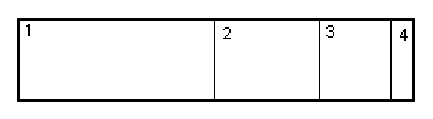
\includegraphics[width=2.5in, height=0.5in]{roulettepic}
\end{center}
\caption{Conceptual roulette "wheel".}
\label{fig_roulette}
\end{figure}
No matter which method is used, the final step is the same -
reshape the vector of chromosome indices into the $\left(
\frac{n}{2},2\right) $ \textcode{parents} matrix.

\subsection*{Example}
\begin{verbatim}
INPUT
rand('state',1975)
fit = sort(rand(10,1),'descend');
S = GAselect(fit,-1,1);
R = GAselect(fit,-1,2);
disp(MatrixtoStr(fit))
disp(MatrixtoStr(S,'%02.0f'))
disp(MatrixtoStr(R,'%02.0f'))
S = GAselect(sort(rand(11,1),'descend'),1,1);
disp(MatrixtoStr(S,'%02.0f'))
OUTPUT
       1         1  2        1  2       1  2
  ----------   -------     -------     -------
 1| 0.75736| 1 |01 02|   1 |01 01|   1 |11 10|
 2| 0.74900| 2 |03 04|   2 |06 01|   2 |11 09|
 3| 0.70559| 3 |05 06|   3 |01 05|   3 |08 07|
 4| 0.65754| 4 |07 08|   4 |01 07|   4 |06 05|
 5| 0.60761| 5 |09 10|   5 |04 03|   5 |04 03|
 6| 0.53533|   -------     -------   6 |02 01|
 7| 0.51611|                           -------
 8| 0.27495|
 9| 0.16207|
10| 0.11422|
  ----------
\end{verbatim}
Here we've already sorted the vector of fitness scores such
that the most fit chromosomes (highest scores).are at the
beginning of the vector. We can see that the sorted method
(first output) seeds the next generation by simply pairing
sequential chromosomes. The top two will be mated, as will the
next two, with the sequence continuing through the entire
population.
However, in the second output, we see that the best solution will be mated $%
5 $ times! For the last computation, we've assumed a population of $n=11$,
and switch to a minimization GA - hence the best solutions are at the end of
the vector. We see that the most fit chromosome was intelligently inserted
into the parent vector, such that it will be mated with the 2$^{\text{nd}}$
and 3$^{\text{rd}}$ best individuals, and not with itself.

\section{Chromosomal Crossover}

\subsection*{Syntax}

\textcode{offspring = GAcrossover(population, parents,
crossover rate, crossover type)}

\subsection*{Description}

Performs chromosomal crossover on the current generation of a GA after the
solutions have been selected and paired for mating.

\subsection*{Input / Output}

\begin{compactitem}

\item \textcode{population} - $\left( n \times p \right)$ matrix of current GA population.

\item \textcode{parents} - $\left( \frac{n}{2} \times 2 \right)$ matrix indicating pairs of solution indices to mate from \textcode{GAselect}.

\item \textcode{crossover rate} - Scalar probability of crossover in $\left[0,1\right]$.

\item \textcode{crossover type} - Scalar indicating type of crossover to perform: 1 =  single point, 2 =  dual point, 3 =  uniform.

\item \textcode{offspring} - $\left( n \times p \right)$ matrix of next GA population.

\end{compactitem}

\subsection*{Algorithm}

There are three methods of crossover implemented by this function, and all
three start by determining if a given mating pair will produce crossed-over
or identical offspring. A random number is generated from the usual uniform
distribution; if it is less than the probability of crossover, the parental
chromosomes are crossed to form the offspring. Otherwise, they are merely
duplicated unchanged.

\begin{compactitem}
\item[single-point] If single-point crossover is selected, an integer in $%
\left[ 1,p\right] $ is selected randomly. The parental chromosomes are then
traded at this point such that the "son" gets the $\left[ 1,X\right]$ portion of the "dad's" chromosome and the $\left[ X+1,p\right] $ portion of
the "mom's" chromosome. The "daughter" binary string is the opposite.

\item[dual-point] In dual-point crossover, two crossover points are randomly
selected, and the parent strings are divided into three portions: $\left[
1,X_{1}\right] $, $\left[ X_{1}+1,X_{2}\right] $, $\left[ X_{2}+1,p\right] $%
. The son inherits the 1$^{\text{st}}$ and 3$^{\text{rd}}$ portions from the
father and the 2$^{\text{nd}}$ from the mother. Again, the daughter is built
out of what's left.

\item[uniform] For the final method, $p$ random uniform variates are
generated, and those that are less than the crossover
probability are trading points. The son is created by taking
the points from the father corresponding to the trading points,
with all others coming from the mother. The daughter is created
in the reverse manner.
\end{compactitem}

\emph{Table \ref{tab_xoverex}} has an example of each of these.
\begin{table}[htbp]
\begin{center}
\begin{tabular}{ccc}
& Crossover Point(s) & Parents $\longrightarrow $Offspring \\
Single & $2$ & $%
\begin{bmatrix}
1 & 1| & 1 & 1 & 1 & 1 \\
0 & 0| & 0 & 0 & 0 & 0%
\end{bmatrix}%
\longrightarrow
\begin{bmatrix}
1 & 1| & 0 & 0 & 0 & 0 \\
0 & 0| & 1 & 1 & 1 & 1%
\end{bmatrix}%
$ \\
Dual & $3,5$ & $%
\begin{bmatrix}
1 & 1 & 1| & 1 & 1| & 1 \\
0 & 0 & 0| & 0 & 0| & 0%
\end{bmatrix}%
\longrightarrow
\begin{bmatrix}
1 & 1 & 1| & 0 & 0| & 1 \\
0 & 0 & 0| & 1 & 1| & 0%
\end{bmatrix}%
$ \\
Uniform & $1,3,5$ & $%
\begin{bmatrix}
1| & 1 & 1 & 1| & 1| & 1 \\
0| & 0 & 0 & 0| & 0| & 0%
\end{bmatrix}%
\longrightarrow
\begin{bmatrix}
1| & 0 & 0| & 1 & 1| & 0 \\
0| & 1 & 1| & 0 & 0| & 1%
\end{bmatrix}%
$%
\end{tabular}%
\end{center}
\caption{Crossover Examples - "$|$" Indicates Crossover Points}
\label{tab_xoverex}
\end{table}

\subsection*{Example}

In this example, we've taken the same population of just two individuals,
and performed crossover using each of the three methods.
\begin{verbatim}
INPUT
rand('state',42)
P = [1,1,0,1,0;1,0,1,0,1];
S = GAcrossover(P,[1,2],1,1);
D = GAcrossover(P,[1,2],1,2);
U = GAcrossover(P,[1,2],0.8,3);
disp(MatrixtoStr(P,'%0.0f'))
disp(MatrixtoStr(S,'%0.0f'))
disp(MatrixtoStr(D,'%0.0f'))
disp(MatrixtoStr(U,'%0.0f'))
OUTPUT
   1 2 3 4 5
  -----------
1 |1 1 0 1 0|
2 |1 0 1 0 1|
  -----------
   1 2 3 4 5       1 2 3 4 5       1 2 3 4 5
  -----------     -----------     -----------
1 |1 1 1 0 1|   1 |1 0 1 1 0|   1 |1 1 0 1 1|
2 |1 0 0 1 0|   2 |1 1 0 0 1|   2 |1 0 1 0 0|
  -----------     -----------     -----------
\end{verbatim}
Here we see that, for the single-point crossover method, $X=2$
was chosen as the crossover point, while $X=\left[ 1,3\right] $
was chosen for the
dual-point crossover. Finally, for the uniform method, the 2$^{\text{nd}}$, 3%
$^{\text{rd}}$, and 4$^{\text{th}}$ points were chosen.

\section{Genetic Mutation}

\subsection*{Syntax}

\textcode{mutated = GAmutation(population, mutation rate)}

\subsection*{Description}

Perform random mutation on a population of chromosomes, this is usually
performed after a generation has mated and produced the next generation.

\subsection*{Input / Output}

\begin{compactitem}

\item \textcode{population} - $\left( n \times p \right)$ matrix of n offspring GA solutions.

\item \textcode{mutation rate} - Scalar probability of mutation in $\left[0,1\right]$.

\item \textcode{mutated} - $\left( n \times p \right)$ matrix of n mutated offspring GA solutions.

\end{compactitem}

\subsection*{Algorithm}

The algorithm for mutation is very simple. The first step is to generate an $%
\left( n\times p\right) $ matrix, $M$, of random numbers drawn
from $U\left( 0,1\right) $, using the Matlab \textcode{rand}
function. Using the logical indexing capability of Matlab, any
loci in the population that correspond to elements of $M$ that
are less than the mutation rate have their bits flipped - a
\textit{not} operation. This function is so simple, the code is
shown here.
\begin{verbatim}
[num_chrom, p] = size(popul);
mutation_chances = mutat_rate > rand(num_chrom,p);
newpop = popul;
newpop(mutation_chances) = not(newpop(mutation_chances));
\end{verbatim}

\subsection*{Example}

We demonstrate how this function with a trivial example. First we create a
GA population with $n=100$ chromosomes all of length $100$; however, all
entries are $0$. Using a mutation rate of $75\%$, we would expect
approximately $7500$ bits to be flipped; in this example, a close 7437 were.
\begin{verbatim}
INPUT
a = zeros(100,100);
mutat_rate = .75;
rand('state',42)
b = GAmutation(a,mutat_rate);
actual = sum(sum(b)
expect = prod(size(a))*mutat_rate
OUTPUT
actual =
        7437
expect =
        7500
\end{verbatim}
Here we have a reasonably realistic example.
\begin{verbatim}
INPUT
rand('state',42)
GAmutation([0,1,1,0,1;0,1,0,0,1],0.10)
OUTPUT
ans =
     0     1     0     0     1
     0     1     0     0     1
\end{verbatim}

\section{GA Engineering}

\subsection*{Syntax}

\textcode{new offspring = GAengineering(previous best, current
best, current offspring, engineer rate)}

\subsection*{Description}

One criticism of the genetic algorithm is that, due to its stochastic
nature, subsequent runs can end up with different solutions to the same
problem. This is typically only a problem if a problem is very large and/or
when the number of generations and population size parameters are set too
low. One solution is to employ GA engineering. This function implements GA
engineering, the point of which is to limit the variability between GA runs.
It takes the best solution from the previous generation and the best
solution from the current generation, and finds the difference. Where they
are different, the bits from the previous best are inserted into the
offspring of the current generation with the specified probability. This
should only be called if the best from the previous generation is better
than the current best.

\subsection*{Input / Output}

\begin{compactitem}

\item \textcode{previous best} - $\left( 1 \times p \right)$ vector holding the chromosome of the best solution from the previous generation.

\item \textcode{current best} - $\left( 1 \times p \right)$ vector holding the chromosome of the best solution from the current generation.

\item \textcode{current offspring} - $\left( n \times p \right)$ matrix of all offspring from the current generation.

\item \textcode{engineer rate} - Scalar probability of engineering in $\left[ 0,1 \right]$.

\item \textcode{new offspring} - $\left( n \times p \right)$ matrix of all offspring from the current generation after being engineered.

\end{compactitem}

\subsection*{Algorithm}

The first step in \textcode{GAengineering} is to identify the
differences between the best solutions of the previous and
current generations, and their indices. Next, a vector of
random probabilities is generated, having the same size as the
next generation. Offspring corresponding with a random variate
being less than the engineer rate have their bits at the
difference indices set to the bit values of the previous
generation best. For example, if the previous and current solutions are $%
\begin{bmatrix}
1 & 0 & 0 & 1 & 0 & 1 & 1 & 1%
\end{bmatrix}%
$ and $%
\begin{bmatrix}
1 & 0 & 1 & 1 & 0 & 0 & 1 & 0%
\end{bmatrix}%
$, respectively, and the previous best had a better score, the bits inserted
into the next generation will be $%
\begin{bmatrix}
\_ & \_ & 0 & \_ & \_ & 1 & \_ & 1%
\end{bmatrix}%
$.

\subsection*{Example}

Here we have an example with only three offspring. As can be seen below, the
1$^{\text{st}}$ and 2$^{\text{nd}}$ members of the next generation had $%
\begin{bmatrix}
\_ & \_ & 0 & \_ & \_ & 1 & \_ & 1%
\end{bmatrix}%
$ inserted into their chromosomes.
\begin{verbatim}
INPUT
pgbest = ([1,0,0,1,0,1,1,1] == 1);
cgbest = ([1,0,1,1,0,0,1,0] == 1);
cgoff = ([ones(1,8);zeros(1,8);...
   [ones(1,4),zeros(1,4)]] == 1);
rand('state',42)
engoff = GAengineering(pgbest, cgbest, cgoff, 0.5);
disp(MatrixtoStr(cgoff))
disp(MatrixtoStr(engoff))
OUTPUT
   1 2 3 4 5 6 7 8
  -----------------
1 |1 1 1 1 1 1 1 1|
2 |0 0 0 0 0 0 0 0|
3 |1 1 1 1 0 0 0 0|
  -----------------
   1 2 3 4 5 6 7 8
  -----------------
1 |1 1 0 1 1 1 1 1|
2 |0 0 0 0 0 1 0 1|
3 |1 1 1 1 0 0 0 0|
  -----------------
\end{verbatim}

\section{GA for Real-valued Function Optimization}

\subsection*{Syntax}

\textcode{[best solution, best score] = GArealoptim(parameters,
number bits, lower bounds, upper bounds, extra plot title,
objective function, up to 5 parameters)}

\subsection*{Description}

This implements the genetic algorithm for optimization of real valued
functions with $p$ parameters. Binary representations, of length $B_{i}$ for
all $p$ parameters are concatenated so that all GA operations are performed
on a single binary string of length $\sum_{i=1}^{p}B_{i}$.

\subsection*{Input / Output}

\begin{compactitem}

\item \textcode{parameters} - $\left( 1 \times 15 \right)$ vector of GA parameters:
\begin{compactenum}

\item \textcode{population size} - Number of chromosomes in each
population.

\item \textcode{number generations} - Maximum number of
generations to perform.

\item \textcode{minimum number generations} -
Number of generations with insufficient improvement for early
termination.

\item \textcode{convergence criteria} - When testing for
early termination, any improvement less than this is deemed to be
none.

\item \textcode{elitism} - Scalar indicating if the best chromosome
cross generations unchanged: 1 = yes, 0 = no.

\item \textcode{generation
seeding type} - Scalar indicating generation seeding method to use, see
\textcode{GAselect}.

\item \textcode{crossover rate} - Scalar probability
of crossover in $\left[ 0,1 \right]$.

\item \textcode{crossover type} -
Scalar indicating type of crossover to perform, see \textcode{GAcrossover}%
.

\item \textcode{mutation rate} - Scalar probability of mutation in $%
\left[ 0,1 \right]$.

\item \textcode{GA engineering rate} - Scalar
probability of GA engineering in $\left[ 0,1 \right]$.

\item \textcode{%
optimization goal} - Scalar indicating which type of optimization to
perform: 1 = maximization, -1 = minimization.

\item \textcode{progress
plot flag} - Scalar indicating when to update the GA progress plot: -1 = no
plot, 1 = with each iteration, 0 = at end.

\item \textcode{3d surface
plot flag} - Scalar indicating whether or not to create a 3-d surface plot
of the objective function: 1 = yes, -1 = no. If \textcode{elitism} is on,
this will be turned off.

\item \textcode{screen output flag} - Scalar
indicating what to print to the screen: -1 = nothing, 0 = summary only, 1 =
summary and with each iteration.

\item \textcode{randomization} - If 0 is
passed, the random state will be set by \textcode{sum(clock()*1000000)},
otherwise, the value passed is used as the state.

\end{compactenum}%


\item \textcode{number bits} - $\left( 1 \times p \right)$ vector with
number of bits used to encode real values.

\item \textcode{lower bounds}
- $\left( 1 \times p \right)$ vector with lower bound of range for real
values.

\item \textcode{upper bounds} - $\left( 1 \times p \right)$
vector with upper bound of range for real values.

\item \textcode{extra
title} - String, extra information to put on plot titles (just [] if not
desired).

\item \textcode{objective function} - String indicating name of
function to optimize

\item \textcode{P1} - Optional secondary parameter
to pass \textcode{objective function}.

\item \textcode{P2} -  Optional
tertiary parameter to pass \textcode{objective function}.

\item \textcode{%
P3} - Optional fourth parameter to pass \textcode{objective function}%
.

\item \textcode{P4} - Optional fifth parameter to pass \textcode{%
objective function}.

\item \textcode{P5} - Optional sixth parameter to
pass \textcode{objective function}.

\item \textcode{best solution} -
Scalar real value that optimized the \textcode{objective function}.

\item
\textcode{best score} - Scalar optimized value of \textcode{objective
function}.

\end{compactitem}

\subsection*{Example}

Here we provide a simple example with the GA trying to find the maximum
likelihood estimators $\hat{a}$ and $\hat{b}$ for the gamma distribution. We
start by generating $n=1000$ samples from $Gamma\left( 2,3\right) $:

\begin{equation}
f\left( x\right) =\frac{1}{b^{a}\Gamma \left( a\right) }x^{a-1}e^{-ax^{b}}%
\text{.}  \label{eqn_gamma}
\end{equation}
\begin{verbatim}
% simulate data
dist = 'GAM'; n = 1000;
reala = 2; realb = 3;
X = SimDistData(dist,n,[reala,realb],42);
% set up for GA
parms = [50,50,10,1e-5,1,2,0.75,1,0.10,0.50,1,0,-1,1,42];
[LB,UB] = EstParamRanges(dist,X);
% run GA
[maxloglike,mles] = GArealoptim(parms,[32;32],...
   LB,UB,dist,'ComputeLogLike',X,dist);
\end{verbatim}
As can be seen below, the GA converged in $2.25$ seconds to $\hat{\alpha}%
=2.003$ and $\hat{b}=2.992$. Given that these parameters are generally taken
to be whole numbers, it's clear that this is equivalent to the true values
of $a=2$ and $b=3$. From \emph{Figure \ref{fig_realGAex}}, we see that the
GA found this solution very quickly - by the 20$^{\text{th}}$ generation or
so.
\begin{figure}[htbp]
\begin{center}
\includegraphics[width=4in]{GAreal_example}
\end{center}
\caption{Sample GA Progress Plot.}
\label{fig_realGAex}
\end{figure}
\begin{verbatim}
GA BEGAN
##################################################
Started on: 20071203_164209
Random State:         42
Maximum # Generations: 50
Minimum # of Generations: 10
Convergence Criteria: 1e-005
Population Size: 50
Crossover Rate: 0.75
Mutation Rate: 0.10
Crossover Method: SINGLE-POINT
Mating Method: ROULETTE
!!With Elitism ON, the probability of GA
   engineering has been set to 0.00!!
Elitism is: ON
Objective: MAXIMIZE
Objective Function: ComputeLogLike
##################################################

Gen 1 of 50: Best = -2672.6021, Early Term = 1
Gen 3 of 50: Best = -2672.6021, Early Term = 3
Gen 5 of 50: Best = -2672.6021, Early Term = 5
...
Gen 31 of 50: Best = -2671.9865, Early Term = 5
Gen 33 of 50: Best = -2671.9865, Early Term = 7
Gen 35 of 50: Best = -2671.9865, Early Term = 9
Early Termination On Generation 36 of 50
Gen 36 of 50: Best = -2671.9865, Early Term = 10

=====================================================
GA Complete
---------------------------------------
              ComputeLogLike Frequency
---------------------------------------
[2.003,2.992]    -2671.987       10
[2.003,2.992]    -2671.987       7
[1.963,3.057]    -2672.205       8
[1.963,3.022]    -2672.314       1
[1.947,3.031]    -2672.602       3
[1.947,3.031]    -2672.602       7
---------------------------------------
=====================================================
GA Completed in
    2.2500 Seconds
    0.0375 Minutes
    0.0006 Hours
\end{verbatim}

\section{GA Subsetting Template}

\subsection*{Syntax}

\textcode{GAtemplate}

\subsection*{Description}

This is a general template used for creating and running the genetic
algorithm for a variable subsetting problem.

\subsection*{Input / Output}

All input is made by modifying the parameters for the GA in the
section of the script with the \textcode{\% initialize model
selection parameters} comment heading.

\begin{compactitem}

\item \textcode{showtopsubs} - Number of best subsets to show in the final summary.

\item \textcode{popul\_size} - Number of chromosomes in each population.

\item \textcode{num\_generns} - Maximum number of generations to perform.

\item \textcode{convgcrit} - When testing for early termination, any improvement less than this is deemed to be none.

\item \textcode{elitism} - Scalar indicating if the best chromosome cross generations unchanged: 1 = yes, 0 = no.

\item \textcode{sel\_type} - Scalar indicating generation seeding method to use, see \textcode{GAselect}.

\item \textcode{prob\_xover} - Scalar probability of crossover in $\left[ 0,1 \right]$.

\item \textcode{xover\_type} - Scalar indicating type of crossover to perform, see \textcode{GAcrossover}.

\item \textcode{prob\_mutate} - Scalar probability of mutation in $\left[ 0,1 \right]$.

\item \textcode{prob\_engineer} - Scalar probability of GA engineering in $\left[ 0,1 \right]$.

\item \textcode{nochange\_terminate} - Number of generations with no improvement in objective to go before early termination.

\item \textcode{objec\_func} - String name of function to be optimized.  The \textcode{feval} line in the code needs to be modified to pass parameters to this function correctly.

\item \textcode{maxmin} - Scalar indicating which type of optimization to perform: 1 = maximization, -1 = minimization.

\item \textcode{pltflg} - Scalar indicating when to update the GA progress plot: 1 = with each iteration, 0 = at end.

\item \textcode{plt3d} - Scalar indicating whether or not to create a 3-d surface plot of the objective function: 1 = yes, 0 = no. If \textcode{elitism} is on, this will be turned off.

\item \textcode{randstate} - If 0 is passed, the random state will be set by \textcode{sum(clock()*1000000)}, otherwise, the value of randstate is used as the state.

\end{compactitem}

No matter what values are entered for \textcode{prob\_engineer}
or \textcode{plt3d}, they will be set to $0.00$ and $0$,
respectively, if the elitism rule is turned on. Output from
\textcode{GAtemplate} is by way of up to four files saved in a
"...\textbackslash output \textbackslash" directory.

\begin{compactitem}
\item GASub\_\%objec\_func\%\_\%time started YYYYMMDD\_HHMMSS\%.mat -
Matlab workspace file storing all parameters, data, and other relevant variables from a replication of
the GA. The relevant variables include:
\begin{compactitem}
\item \textcode{GA\_BEST} - A matrix holding the unique best results from
all generations. The first column holds the fitness scores,
the second has the number of generations that had that
score as the best, and the rest of the columns are occupied
by the solution chromosome associated with that score. The
rows are sorted with the best results at the top.

\item \textcode{allscores} - A matrix storing all fitness scores for all
generations - this is only created if the 3-d surface plot
is.

\item \textcode{save\_prefix} - A character string holding the identical
prefix used for saving all the files.

\item \textcode{ga\_toc} - The time in seconds required by the
GA.
\end{compactitem}


\item GASub\_\%objec\_func\%\_\%time started YYYYMMDD\_HHMMSS\%.out - Text
file storing GA progress and summary information printed into
the Matlab command window.

\item GASub\_\%objec\_func\%\_\%time started YYYYMMDD\_HHMMSS\%\_GA.fig -
Matlab figure file with GA progress plot showing the optimum
score and average score from each generation.

\item GASub\_\%objec\_func\%\_\%time started YYYYMMDD\_HHMMSS\%\_3d.fig -
Matlab figure file 3-dimensional surface plot of objective
function - plotted with population on the X axis and generation
on the Y axis (only created and saved if \textcode{plt3d} is on
and \textcode{elitism} is off.
\end{compactitem}

An obvious and well-asked question is why isn't the input through a GUI.
This script was designed to be able to be run from a script that would
perform multiple replications or a Monte Carlo experiment, with little
modification. It wouldn't make sense to have to fill in some kind of GUI
with the same data $1000$ times! Additionally, while we could have also made
it a function, rather than a script, we wanted to make a lot of variables
available as output - it wouldn't make sense to have an output argument list
with 20 or 30 items.

\subsection*{Algorithm}

Variable subsetting is a statistical modeling problem that lends itself to
the genetic algorithm very well. Consider some multivariate data $X\in
\mathbb{R}^{n\times p}$, can we reduce the dimensionality of the data into $%
q $ dimensions, with $q<p$? One context in which this is commonly a goal is
regression - redundant covariates can have a negative effect on the least
squares fit (see \emph{Chapter 13 - Multivariate Regression}). If $p$ is
small, it is a simple manner to evaluate all possible subsets; for $p=5$,
for example, there are $2^{5}-1=31$ ways to combine the five variables.
However, as $p$ increases linearly, the number of possible subsets increases
exponentially. Consider $p=8$, there are $255$ subsets models to evaluate.
This where the GA can be a powerful tool. To cast the subsetting problem
with $p=8$ into the GA framework, consider a possible solution string $%
\begin{bmatrix}
1 & 0 & 0 & 1 & 1 & 1 & 0 & 0%
\end{bmatrix}%
$ - if we use this for logical indexing of $X$ in Matlab, the subset model
includes variables $\left[ 1,4,5,6\right] $.

The \textcode{GAtemplate} script is an all-purpose GA
implementation for this subsetting problem. Code can be
inserted to do any data loading or preparation desired, and the
objective function can be changed with only one real
limitation. No matter how many out arguments it uses, the first
must be the fitness score. Of course, with some coding, this
can be bypassed. As written, this script can solve both
maximization and minimization problems. \textcode{GAtemplate}
follows the general GA flow as detailed in the introduction.
Upon completion of the iterative procedure, the appropriate
plots are created and saved and the best \textcode{showtopsubs}
unique solutions and the associated scores from all generations
are displayed in a table.

\subsection*{Example}

We demonstrate this script with the familiar body fat dataset. This data is
composed of body measurement observations from $n=252$ men. There are $p=13$
regressors, listed in \emph{Table \ref{tab_body}} - note that the two
responses have been left off. Where not specified, measurements are in
centimeters.
\begin{table}[htbp]
\begin{center}
\begin{tabular}{cc}
$x_{1}=$Age (yrs) & $x_{2}=$Weight (lbs) \\
$x_{3}=$Height (in) & $x_{4}=$Neck circumference \\
$x_{5}=$Chest circumference & $x_{6}=$Abdomen 2 circumference \\
$x_{7}=$Hip circumference & $x_{8}=$Thigh circumference \\
$x_{9}=$Knee circumference & $x_{10}=$Ankle circumference \\
$x_{11}=$Extended biceps circumference & $x_{12}=$Forearm circumference \\
$x_{13}=$Wrist circumference &
\end{tabular}%
\end{center}
\caption{Body fat dataset variables.}
\label{tab_body}
\end{table}
We ran \textcode{GAtemplate} five times using the parameters
shown here (from the final run).
\begin{verbatim}
##############################################
\output\GASub_MVGaussLogLike_20071128_095157
Started on: 20071128_095157
Random State: 2163062000
Maximum # Generations: 50
Minimum # of Generations: 30
Convergence Criteria: 0
Population Size: 30
Crossover Rate: 0.75
Mutation Rate: 0.10
Crossover Method: SINGLE-POINT
Mating Method: ROULETTE
GA Engineering Rate: 0.00
Elitism is: ON
Objective: MAXIMIZE
Objective Function: MVGaussLogLike
\data\BodyFatData.m
##############################################
\end{verbatim}
There are a total of $2^{13}-1=8191$ subsets; one run of the
genetic algorithm will evaluate, unless it terminates early, at
most $30\ast 50=1500$ solutions. Recall that there is no
artificial constraint to prevent the GA from reevaluating
subsets. Thus, at most $18.3\%$ of the subspace will be
evaluated. As can be seen, the objective here is to find the
subset that maximizes the multivariate Gaussian log likelihood.
We are not claiming that this is a good model for this data. In
fact, the tests for multivariate Gaussian kurtosis and skewness
implemented in \textcode{MVNormalityTest}
both strongly reject the null hypothesis of Gaussianity with p-values $%
<0.00000$. Partial output from the final run is shown below, and the
progress plot is shown in \emph{Figure \ref{fig_gaprogplt}}.
\begin{verbatim}
==============================================
GA Complete
------------------------------
     MVGaussLogLike Frequency
------------------------------
{13}    -339.754        10
{12}    -534.339        24
{4}     -580.916        16
------------------------------
==============================================
GA Completed in
    1.5780 Seconds
    0.0263 Minutes
    0.0004 Hours
\end{verbatim}
\begin{figure}[htbp]
\begin{center}
\includegraphics[width=4in]{GASub_MVGaussLogLike_20071128_095157_GA}
\end{center}
\caption{GA Progress Plot from Final Run.}
\label{fig_gaprogplt}
\end{figure}
These results were typical of all $5$ runs - all selected the subset with
only $x_{13}=$ Wrist circumference. The same tests for normality applied to
this subset were unable to reject the null hypothesis that the data came
from a normal distribution, as seen in \emph{Figure \ref{fig_mvnorm13}}.
\begin{figure}[htbp]
\begin{center}
\includegraphics[width=\textwidth]{Subset13_MVGaussTest}
\end{center}
\caption{Normality Test Plots for Best Subset.}
\label{fig_mvnorm13}
\end{figure}
To show that this is actually a good solution, we wrote a
second script, \textcode{evalusubs\_bodyfat}, to compute the
same objective function for all $8191$ subsets of the body fat
data and display the best $10$. As can be see below, the GA
honed in on the best subset; additionally, the other two
solutions selected by any of the $50$ generations were also in
the top five. Thus we've demonstrated here that by only looking
at $18.3\%$ of the subset space (at most), the stochastic
search performed as well as the much more computationally
intensive all-subsets approach.
\begin{verbatim}
-----------------------
        MVGaussLogLike
-----------------------
{13}       -339.754
{10}       -490.033
{12}       -534.339
{9}        -578.927
{4}        -580.916
{11}       -635.703
{3}        -684.230
{8}        -774.944
{10,13}    -782.087
{4,13}     -819.716
-----------------------
\end{verbatim}

\section{GA Parametric Model Estimation and Fitting}

\subsection*{Syntax}

\textcode{drv\_GAMLE}

\subsection*{Description}

Use the real-valued genetic algorithm to estimate parameters for various
distributions fit to either simulated or real data, then use information
criteria to pick the best model. This is a very flexible script, allowing
the user to control the output, modify GA parameters, select the
distribution (out of many) from which to simulate, and select a subset of
distributions to fit.

\subsection*{Input / Output}

\begin{figure}[htbp]
\begin{center}
\includegraphics[width=\textwidth]{drvGAMLE_flow}
\end{center}
\caption{\textcode{drv\_GAMLE} Flow Diagram.}
\label{fig_flow}
\end{figure}
The flow diagram in \emph{Figure \ref{fig_flow}} identifies the sequence of
activities in this script in general. Specifically of interest are the boxes
with bold outlines. These are where the user provides input - either by a\
pop-up dialogue window, or through the command window. All of the parameters
have been discussed elsewhere in this chapter, except for the Information
Criteria (IC on flow). The current two choices are \emph{AIC} and \emph{SBC}%
, shown in \emph{equations \ref{eqn_SBC}} and \emph{\ref{eqn_AIC}},
respectively.

All output is by way of screen output, which is saved into a
Matlab diary file, and possibly several plots. Everything that
is printed to the Matlab command window is saved into a
human-readable text file named "GAMLE\_\%time started
YYYYMMDD\_HHMMSS\%", saved in the directory in which the script
resides. If the user has set the screen output flag to $0$ or
$1$, this will include output from \textcode{GArealoptim} as
appropriate. If either of the plotting flags (progress plot,
surface plot) were not set to $-1$, these plots will be created
- one per distribution fit per simulation. Be careful
with the plotting flags, up to $11$ distributions can be fit to data; for $%
10 $ simulations, that's $110$ GA progress plots. Finally, a density
histogram of the data - either the real data, or the final simulation - is
constructed, and the overall best probability density function is overlaid.

\subsection*{Algorithm}

For a parametric model, the two information criteria used by \textcode{%
drv\_GAMLE}\ are shown below.

\begin{equation}
AIC=-2\log l\left( \hat{\theta}\mid X\right) +2p  \label{eqn_AIC}
\end{equation}

\begin{equation}
SBC=-2\log l\left( \hat{\theta}\mid X\right) +p\log n  \label{eqn_SBC}
\end{equation}

Here, $\hat{\theta}$ indicates the maximum likelihood
estimators determined by the GA, and $p$ indicates the number
of parameters estimated. You'll note on the flow diagram that
one of the steps indicates the fitting distributions could be
subset by the script. In the case of simulated data that could
include negative values (such as $N\left( 0,1\right) $), or
real data that actually includes negative values, it doesn't
make sense to fit strictly positive distributions, such as
$\chi ^{2}$ to the data. \textcode{drv\_GAMLE} figures this out
by looking at the outputs returned by
\textcode{ComputeLogLike}\ when no parameters are passed in.

One quirk that should be mentioned - \textcode{GArealoptim}
knows nothing of the usual limitations on some distributional parameters, such as $%
\sigma >0$ or $\nu \in \mathbb{N}$. Thus, it could very well
optimize the Student's t with 3.65 degrees of freedom.

\subsection*{Example}

We demonstrate this script using the first variable of the body fat data
already used in this chapter - $x_{1}=$ age in years. The parameters used
shown in the output below.
\begin{verbatim}
@@@@@@@@@@@@@@@@@@@@@@@@@@@@@@@@@@@@@@@@@@@@@@@@@@@@
drv_GAMLE began on 20071205_100557
----------------------------------------------------
NRM(mu,sigma): [45.02 12.87]: AIC = 1995.5015
GAM(a,b): [12.37 3.63]: AIC = 1989.5399
LOG(mu,sigma): [3.76 0.27]: AIC = 1997.7414
EXP(b): [44.82]: AIC = 2423.2678
WEI(a,b): [0.03 0.11]: AIC = 3724.7374
CHI(nu): [44.07]: AIC = 2042.6860
STU(nu): [0.22]: AIC = 3580.4350
CAU(theta): [43.30]: AIC = 2544.7308
LPL(mu,sigma): [43.33 5.12]: AIC = 2019.4872
PXP(mu,sigma,beta): [45.62 16.38 1.50]:
   AIC = 1996.0318
PAR(c): [0.26]: AIC = 3085.7170
BEST MODEL: GAM
----------------------------------------------------
====================================================
-GA Parameters-
Population Size: 50
Maximum # Generations: 50
Minimum # of Generations: 10
Convergence Criteria: 1e-005
Elitism is: OFF
Mating Method: ROULETTE
Mutation Rate: 0.10
Crossover Rate: 0.75
Crossover Method: SINGLE-POINT
GA Engineering Rate: 0.50
Randomizer:          0
Encoding Rate: 32
-Data Parameters-
Fit data in \data\BodyFatData.m
Number Observations: 252
====================================================
AIC Values
-----------------------------------------------
  NRM     GAM     LOG     EXP     WEI     CHI
-----------------------------------------------
1995.50 1989.54 1997.74 2423.27 3724.74 2042.69
-----------------------------------------------
-----------------------------------------
   STU   CAU     LPL     PXP     PAR
-----------------------------------------
 3580.43 2544.73 2019.49 1996.03 3085.72
------------------------------------------

Best Overall Model:
GAM(a,b): [12.37 3.63]: AIC = 1989.5399
Modeling Completed in
    14.1880 Seconds
    0.2365 Minutes
    0.0039 Hours
Diary file saved:GAMLE_20071205_100557.out
@@@@@@@@@@@@@@@@@@@@@@@@@@@@@@@@@@@@@@@@@@@@@@@@@@@@
\end{verbatim}
From the final summary, we see that the distribution that best
fit this data was the gamma distribution, with the Gaussian
distribution a close second choice. Of course, we'd probably
round the parameters of the gamma distribution to $\hat{a}=12$
and $\hat{b}=3.5$, or something. Note that the script didn't
even require a quarter of a minute to use the GA to optimize
the fit of $11$ distributions to the $n=252$ observations. Here
we show the histogram of the data with the best model overlaid,
and the 3-d log likelihood surface plot of the best model.
\begin{figure}
\begin{center}
\subfloat[Data with Best Model]{\includegraphics[width = 2.5in]{bodyfat_age_bstmod}}
\subfloat[Likelihood Surface]{\includegraphics[width = 2.5in]{bodyfat_age_bstsurf}}
\end{center}
\caption{Plots from Fitting Best Gamma Model to Body Fat Age Data.}
\end{figure}

\section{Finding MLEs with Simulated Annealing}

\subsection*{Syntax}

\textcode{[MLE, maximized likelihood] = SimAnneal\_MLE(initial
estimates, parameter limits, data, distribution, parameters)}

\subsection*{Description}

This implements an adaptive simulated annealing algorithm to
find the maximum likelihood estimate(s) for the parameter(s) of
certain distributional models.

\subsection*{Input / Output}

\begin{compactitem}

\item \textcode{initial estimates} - $\left( 1 \times p \right)$ vector of initial estimates for MLEs.

\item \textcode{parameters limits} - $\left( 1 \times p \right)$ vector describing limits on parameters:
\begin{compactitem}
\item -1 = none
\item 0 = nonnegative
\item 1 = strictly positive
\end{compactitem}

\item \textcode{data} - $\left( n \times 1 \right)$ vector of
data.

\item \textcode{distribution} - Character code of distribution
to use, from \textcode{ComputeLogLike}.

\item \textcode{parameters} - $\left( 1 \times 5 \right)$ vector
of parameters:
\begin{compactenum}
\item beginning temperature (very problem dependent)
\item maximum number of iterations
\item randomization code: -1 = none, 0 = auto, else = pass in
state
\item screen output flag: 0 = no, 1 = yes
\item progress plot flag: 0 = no, 1 = yes
\end{compactenum}

\item \textcode{MLE} - $\left( 1 \times p \right)$ vector holding optimal parameter estimates.

\item \textcode{maximized likelihood} - Scalar value of likelihood evaluated at \textcode{MLE}.

\end{compactitem}

\subsection*{Algorithm}

\textcode{SimAnneal\_MLE} employs a temperature schedule such
that the temperature in iteration $k$ is
$T_k=exp\left(-ck^{\frac{1}{p}} \right)$, where $p$ is the
dimension of the function space (number parameters estimated);
we use $c=1$. SA with this temperature schedule is called
Adaptive Simulated Annealing (ASA). If a cooling schedule of
$T_k=\frac{T_0}{k}$, is used, the process is called Cauchy
Annealing. Boltzmann Annealing uses
$T_k=\frac{T_0}{log\left(k\right)}$. Selection of $T_0$ is
crucial to success of the procedure, as it is used in computing
the probability with which the current state is moved to one
with higher energy. If this "bad" move was never allowed, the
SA algorithm works just like a greedy algorithm. The way
simulated annealing is designed, as the temperature decreases,
the probability of making a bad move goes to $0$. The idea is
that when the temperature is high, we want to search enough of
the state space so that as cooling occurs, we end up near a
global optimum. \emph{Figure \ref{fig_samove}} demonstrates how
states evolve.
\begin{figure}[htbp]
\begin{center}
\includegraphics[width=4in]{SA_moveplot}
\end{center}
\caption{Simulated Annealing State Change Plot.}
\label{fig_samove}
\end{figure}
If the energy of the current state, $E_k$, is less than the
energy of the previous state, $E_(k-1)$, the algorithm moves to
the current state. However, if $E_k > E_(k-1)$, a test value is
computed as in \emph{equation \ref{eqn_saprobbad}}.

\begin{equation}
exp(-frac{E_k - E_(k-1)}{T_k})  \label{eqn_saprobbad}
\end{equation}

If this test value is larger than a random variate drawn from
$U\left(0,1\right)$, the algorithm moves to the current state.
The question of how to generate neighboring states can be
problem dependent. For our problem here, we've opted to
generate neighbors based on a multivariate Gaussian
distribution with $\Sigma=2*I_p$, centered at the state of the
previous timestep.

\begin{equation}
f\left( x_{i}\mid \mu ,\Sigma \right) =\left( 2\pi \right) ^{-\frac{p}{2}%
}\left\vert \Sigma \right\vert ^{-\frac{1}{2}}\exp \left( -\frac{1}{2}\left(
x_{i}-\mu \right) ^{\prime }\Sigma ^{-1}\left( x_{i}-\mu \right) \right)
\label{eqn_multnorm}
\end{equation}


\subsection*{Example}

The script \textcode{DemoSAMLE} was written to demonstrate this
function. It generates data from four distributions, and
attempts to optimize their respective log likelihoods.

\begin{tabular}{ccc}
Distribution & Initial Values & Starting Temperature\\
$N\left(\mu=5,\sigma=2\right)$ & $\left[-20,0.25\right]$ & 100000\\
$\chi^2\left(\nu=3\right)$ & $50$ & 10000\\
$Gamma\left(a=2,b=0.5\right)$ & $\left[5,5\right]$ & 100000\\
$PE\left(\mu=-3,\sigma=2,\beta=\frac{1}{2}\right)$ & $\left[-2,1.5,0.25\right]$ & 100
\end{tabular}

To it's credit, SA's dependence on the initial conditions, a
problem in most gradient search methods, seems limited to the
number of iterations required.  However, the method does seem
to be very dependent upon the initial temperature. The correct
temperature seems to be related to both the dimension of the
parameter space and the complexity of the problem. We also
noted a strong effect of the stochastic nature of the
algorithm. It's performance does not seems to be very
consistent. With the exception of the power exponential
distribution, ASA performed admirably. Partial screen output is
shown below.
\begin{verbatim}
NORMAL
----------------
      mu  sigma
----------------   Maximized Log Likelihood at
True 5.00  2.00      True = -2068.249
MLE  5.14  2.16      MLE = -2082.210
----------------
CHI SQUARED
----------
      nu
----------   Maximized Log Likelihood at
True 3.00      True = -2093.888
MLE  3.08      MLE = -2094.284
----------
GAMMA
---------------
       a    b
---------------   Maximized Log Likelihood at
True 2.00 0.50      True = -884.650
MLE  1.66 0.58      MLE = -892.912
---------------
POWER EXPONENTIAL
----------------------
       mu  sigma beta
----------------------   Maximized Log Likelihood at
True -3.00  2.00 0.50      True = -3163.200
MLE  13.84 39.99 6.41      MLE = -4396.184
----------------------
\end{verbatim}
Despite the very close starting values, and experiments with
the initial temperature, we could not get the ASA function to
end up with parameter estimates anywhere near the true values
for the PE distribution. Selected plots are shown in
\emph{Figures \ref{fig_nrmSA}} and \emph{\ref{fig_chiSA}}.
\begin{figure}
\begin{center}
\subfloat[Data with Best Model]{\includegraphics[width = 2.5in]{SA_normfit}}
\subfloat[Likelihood Progress]{\includegraphics[width = 2.5in]{SA_normprog}}
\end{center}
\caption{Plots from Fitting Best Gaussian Model.}
\label{fig_nrmSA}
\end{figure}
\begin{figure}
\begin{center}
\subfloat[Data with Best Model]{\includegraphics[width = 2.5in]{SA_chifit}}
\subfloat[Likelihood Progress]{\includegraphics[width = 2.5in]{SA_chiprog}}
\end{center}
\caption{Plots from Fitting Best $\chi^2$ Model.}
\label{fig_chiSA}
\end{figure}

\end{document}
